\chapter{Probabilistic model checking}
We use Discrete-time Markov chain as the formalism to model stochastic population process. In this
chapter, we present essential concepts on probabilistic model checking, including probabilistic
models and properties. We also briefly present a general deterministic model checking algorithm for
a specific temporal logic, namely PCTL. Due to the state space explosion, applying deterministic
model checking algorithm is possible to be computationally expensive. Therefore, we also present a
simulation based model checking, namely \textit{statistical model checking} for bounded and
unbounded path property. Since statistical model checking relies only on simulation of stochastic
models, it is advantageous for checking models with large space size. We also introduce definitions
of parametric model and parameter synthesis problems, as well as the symbolic computing approach to
verify parametric models.


\section{Markov models}
\subsection{Discrete Time Markov chain}
Markov models are stochastic models of discrete or continous time which satisfy memoryless property.
\begin{definition}[Discrete-time memoryless property]
    Let $X$ be a random variable of geometric distribution. $X$ has memoryless property if and only if
    \begin{align*}
        Pr(X = t + m | X > m) = Pr(X > m) \forall t,m \in \mathbb{N} k \geq 1
    \end{align*}
\end{definition}
Markov model can be non-deterministic \textit{(Markov Decision Process)}. However, in this thesis we
consider only Markov models without non-determinism. The following definitions of discrete-time and
continuous-time Markov chains follows the definitions presented by Baier \cite{baier2008principles}.
\begin{definition}[Discrete Time Markov Chain]
    A Discrete-time Markov chain (DTMC) $\mathcal{M}$ is a tuple $(S,\mathbf{P}, \iota_{init}, AP, L)$,
    in which
    \begin{itemize}
        \item $S$ is a countable, non-emty set of \textit{states}
        \item $\mathbf{P}:S\times S \rightarrow [0,1]$ is the \textit{transition probability}
              function such that
              \begin{align*}
                  \forall s \in S : \sum_{s'\in S}\mathbf{P}(s, s') = 1
              \end{align*}
        \item $\iota_{init}: S \rightarrow [0,1]$ is the \textit{initial distribution} such that
              \begin{align*}
                  \sum_{s\in S} \iota_{init}(s) = 1
              \end{align*}
        \item $AP$ is a set of \textit{atomic propositions}.
        \item $L: S \rightarrow 2^{AP}$ is the labelling function on states.
    \end{itemize}
\end{definition}

\begin{example}[Knuth-Yao die]
    Knuth-Yao die to simulate a 6-faced die by a fair coin. In this Knuth's die DTMC, there are 6
    BSCCs, each of them represents an outcome of a die tossing. Image taken from
    \cite{katoen2016probabilistic}
    \begin{figure}[H]
        \centering
        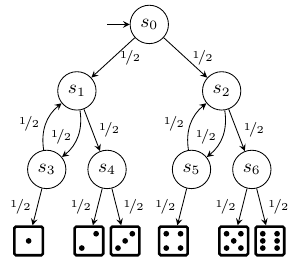
\includegraphics[width=0.5\textwidth]{figures/knuth_die.png}
        \label{fig:knuth-die}
    \end{figure}
\end{example}

\begin{definition}[Strongly Connected Component]
    Let $\mathcal{M}=(S,\mathbf{P}, \iota_{init}, AP,L)$ a DTMC. A subset $S'\subset S$ is strongly
    connected if and only if for every pair $s_1,s_2\in S'$ there is a path between $s_1$ and $s_2$
    which consists of only of state in $S'$. If there exist no $S''\subseteq S$, such that $S\subset
        S''$ and $S''$ is strongly connected, then $S'$ is a \textit{Strongly Connected Component}, or
    \textit{SCC} in short.
\end{definition}

\begin{definition}[Bottom Strongly Connected Component]
    Let $\mathcal{M}=(S,\mathbf{P}, \iota_{init}, AP,L)$ a DTMC and $S'\in S$ a Strongly Connected
    Component. $S'$ is also a \textit{Bottom Strongly Connected Component}, or \textit{BSCC} for
    short, if and only if there exist no state $s \in S\\S'$ that is reachable from any state in
    $S'$. If $|S'|=1$ then $S'$ is a \textit{trivial BSCC}. We denote $BSCC(\mathcal{M})\in S$ is
    the set of all BSCCs of $\mathcal{M}$.
\end{definition}
Intuitively, BSCCs are arbsobing; once a path in a DTMC reaches a state in a BSCC, it visits  all
states in the BSCC infinitely often. It is proven by \cite{baier2008principles} that any run on a
DTMC $\mathcal{M}$ ends in $BSCC(\mathcal{M})$ almost surely.
\begin{theorem}[Long-run theorem]
    Let $\mathcal{M}=(S,\mathbf{P}, \iota_{init}, AP,L)$ a DTMC.
    \begin{align*}
        Pr(\Diamond BSCC(\mathcal{M})) = 1
    \end{align*}
\end{theorem}

In this thesis we concern the \textit{steady-state distribution} of a DTMC.
\begin{definition}[Steady-state distribution]
    Let $\mathcal{M}=(S,\mathbf{P}, \iota_{init}, AP,L)$ a DTMC and vector $v_t$ be a transient state distribution
    \begin{align*}
        v_t = (Pr(X_t=s_1),\ldots,Pr(X_t=s_N)), s_0,\ldots,s_N \in S
    \end{align*}
    A transient state distribution $v$ of $\mathcal{M}$ is a steady-state distribution of $\mathcal{M}$ if and only if
    \begin{align*}
        v = vP
    \end{align*}
\end{definition}
As a result from long-run theorem, if $BSCC(\mathcal{M})\neq \emptyset$ then there exists a
steady-state distribution $v = (Pr(X=s_1),\ldots,Pr(X=s_{|S|}))$, such that
\begin{align*}
    \forall 1 \leq i \leq |S|: P[X=s_i] \neq 0 \Leftrightarrow s_i \in BSCC(\mathcal{M})
\end{align*}


\subsection{Continuous-time Markov chain}
The discrete-time memoryless property can also be extended into continuous-time memoryless property.
In continous-time, memoryless property has the following form
\begin{definition}[Continuous-time memoryless property]
    Let X be a continuous random variable of exponentially distribution. X has memoryless property
    if and only if
    \begin{align*}
        Pr(X > t + \delta | X > t) = Pr(X > \delta), \forall t,\delta \in \mathbb{R}_{\geq 0}
    \end{align*}
\end{definition}
Based on continuous-time memory less property, we introduce the definition of \textit{Continous-time
    Markov chain} \cite{katoen2013model}.
\begin{definition}[Continuous-time Markov chain]
    A Continuous-time Markov chain (CTMC) $\mathcal{C}$ is a tuple $(S,\mathbf{P}, \mathbf{r}, \iota_{init}, AP, L)$
    \begin{itemize}
        \item $S$ is a countable, non-emty set of \textit{states}
        \item $\mathbf{P}:S\times S \rightarrow [0,1]$ is the \textit{transition probability}
              function such that
              \begin{align*}
                  \forall s \in S : \sum_{s'\in S}\mathbf{P}(s, s') = 1
              \end{align*}
        \item $\mathbf{r}:S \rightarrow \mathbb{R}_{>0}$ is the \textit{exit rate} function
              such that
              \begin{align*}
                  \forall s \in S : \sum_{s'\in S}\mathbf{P}(s, s') = 1
              \end{align*}
        \item $\iota_{init}: S \rightarrow [0,1]$ is the \textit{initial distribution} such that
              \begin{align*}
                  \sum_{s\in S}\iota_{init}(s) = 1
              \end{align*}
        \item $AP$ is a set of \textit{atomic propositions}
        \item $L: S \rightarrow 2^{AP}$ is the labelling function on states.
    \end{itemize}
\end{definition}

\begin{example}[CTMC]
    An example of a CTMC with 3 states.
    \begin{figure}[H]
        \centering
        \begin{tikzpicture}[->, >=stealth', auto, semithick, node distance=3cm]
            \tikzstyle{every state}=[fill=white,draw=black,thick,text=black]
            \node[initial, state, label=above:2]    (S0)                   {$S_0$};
            \node[state, label=above:4]    (S1)[right of=S0]      {$S_1$};
            \node[state, label=above:3]    (S2)[right of=S1]      {$S_2$};
            \path

            (S0)
            edge [bend left=20] node{$1$} (S1)

            (S1)
            edge [bend left=20] node{$\frac{2}{3}$} (S2)
            edge [bend left=20] node{$\frac{1}{3}$} (S0)

            (S2)
            edge [bend left=20] node{$1$} (S1);
        \end{tikzpicture}
        \label{fig:ctmc}
    \end{figure}
    \label{example:ctmc}
\end{example}

Continous-time Markov chain has a wide range of applications, especially in bioinformatics where
chemical reaction network \cite{feinberg1980chemical} \cite{anderson2011continuous}. However, the
frameworks in this thesis apply for discrete-time Markov models, thus we do not use continuous-time
Markov chain to model systems of interest directly. Instead, we do not use Continuous-time Markov
models directly. Instead, we transform CTMCs into DTMCs through uniformization \cite{katoen2016probabilistic}
\begin{definition}[CTMC Uniformization]
    Let $\mathcal{C} = (S,\mathbf{P}, \mathbf{r}, \iota_{init}, AP, L)$ be a CTMC. We define the
    \textit{uniformization rate} $r$ such that
    \begin{align*}
        \forall s\in S: r \geq \mathbf{r}(s), r\in\mathbb{R}_{>0}
    \end{align*}
    The \textit{uniformized CTMC} $unif(r, \mathcal{C})=(S, \bar{\mathbf{P}}, \bar{\mathbf{r}}, \iota_{init}, AP, L )$ such that
    \begin{align*}
        \forall s\in S     & : \bar{\mathbf{r}}(s)     \\
        \forall s, s'\in S & : \bar{\mathbf{P}}(s,s')=
        \begin{cases}
            \frac{\mathbf{r}(s)}{r}\mathbf{P}(s,s')                               & \text{if $s \neq s'$} \\ \quad \\
            \frac{\mathbf{r}(s)}{r}\mathbf{P}(s,s') + 1 - \frac{\mathbf{r}(s)}{r} & \text{if $s = s'$}
        \end{cases}
    \end{align*}
\end{definition}

\begin{example}[Uniformized CTMC]
    We uniformize the CTMC in Example \ref{example:ctmc} by uniformization rate $r=4$.
    \begin{figure}[H]
        \centering
        \begin{tikzpicture}[->, >=stealth', auto, semithick, node distance=3cm]
            \tikzstyle{every state}=[fill=white,draw=black,thick,text=black]
            \node[initial, state, label=above:4]    (S0)          {$S_0$};
            \node[state, label=above:4]    (S1)[right of=S0]      {$S_1$};
            \node[state, label=above:4]    (S2)[right of=S1]      {$S_2$};
            \path

            (S0)
            edge [bend left=20] node{$\frac{1}{2}$} (S1)

            (S1)
            edge [bend left=20] node{$\frac{2}{3}$} (S2)
            edge [bend left=20] node{$\frac{1}{3}$} (S0)

            (S2)
            edge [bend left=20] node{$\frac{3}{4}$} (S1);
        \end{tikzpicture}
        \label{fig:uniformized-ctmc}
    \end{figure}
\end{example}
It has been shown by Katoen \cite{katoen2013model} that uniformization preserves the transient
probability distributions. Furthermore, in this thesis we concern steady state data and state
property, thus uniformizing exit rate does not affect the validity of our constructed frameworks.

\section{Property specification}
\subsection{Probabilistic Computational Tree Logic}
Model checking verifies a formalism of a system \textit{(model)} against a property of interest. We
formalize a property by a \textit{temporal logic}, specifically \textit{Probabilistic Computational
    Tree Logic} (or \textit{PCTL}). Firstly introduced by Clarke et al. \cite{clarke1986automatic}, PCTL
is widely used in model checking of discrete-time stochastic models and supported by most
probabilistic model checking tools \cite{dehnert2017storm}, \cite{kwiatkowska2011prism}.
\begin{definition}[PCTL] The syntax of PCTL consists of state formulas and path formulas.
    \begin{itemize}
        \item State formulas are defined over $AP$
              \begin{align*}
                  \Phi & ::= \text{true} \;|\; a \;|\; \Phi \;|\; \Phi_1 \wedge \Phi_2 \;|\; \Phi_1 \vee \Phi_2 \;|\;  P_{J}(\phi)
              \end{align*}
              where $a\in AP$, $\phi$ is a path formula, and $J\subseteq[0,1]$ is an interval.
        \item Path formulas
              \begin{align*}
                  \phi & ::= \bigcirc \Phi \;|\; \Phi_1 \mathsf{U} \Phi_2 \;|\; \Phi_1 \mathsf{U}^{\leq n} \Phi_2
              \end{align*}
              where $\Phi,\Phi_1,\Phi_2$ are state formulas, and $n\in \mathbb{N}$.
    \end{itemize}
\end{definition}
PCTL properties is applicable on discrete-time stochastic models such as DTMC, as the times between
state transitions are uniform. In a DTMC, a PCTL state formula is verified at each state, while a
PCTL path formula is verified through a trace from an execution path.\\
The algorithm to model check DTMC against PCTL properties is described in detail in Katoen
\cite{baier2008principles}. Given a DTMC $\mathcal{M}$ and a PCTL property $\Phi$, general algorithm
for checking $\mathcal{M}\models\Phi$ has complexity of polynomial to $|\mathcal{M}|$ and linear to
$|\Phi|$ \cite{katoen2013model}.
\begin{theorem}[Complexity of checking a DTMC against a PCTL formula.]
    For finite DTMC $\mathcal{M}$ and PCTL state-formula $\Phi$,the PCTL model-checking problem can be solved in time
    \begin{align*}
        \mathcal{O}(poly(size(D)\cdot n_{max} \cdot |\Phi|)
    \end{align*}
    where
    \begin{align*}
        n_{max} =
        \begin{cases}
            max(n | (\Psi_1 \mathsf{U}^{\leq n} \Psi_2) \quad\text{occurs in}\quad \Phi) \\
            1 \text{ if $\Phi$ contains no bounded until property}
        \end{cases}
    \end{align*}
\end{theorem}

\subsection{State exlosion problem}
The soundness of the model checking relies heavily on how the system is modeled. In fact, the model
checking is only as sound and valid as the model.
\begin{enumerate}
    \item Which formalism is used?
    \item How the system is encoded into states and transitions?
\end{enumerate}
For example, we consider a distributed software system, in which a \textit{global state} is a
composition of
\begin{enumerate}
    \item values of all variables, and
    \item states of all communication channels.
\end{enumerate}
It is obvious that the number of possible states grows exponentially as more variables and
communication channels are added to the system.\\
\textit{State-explosion problem} occurs when the size of the system state space grows exponentially
as the number of state variables in the system increases \cite{clarke2011model}. As discussed
before, the complexity of model checking a PCTL property against a DTMC model is polynomial to the
DTMC's state-space. However, the state-explosion problem renders model checking computationally
expensive. One possible way to cope with state-explosion problem and to reduce the computational cost is to use \textit{statistical model
    checking}.

\section{Statistical Model checking}
Statistical model checking is a simulation-based approach to model check a stochastic model
$\mathcal{D}$ against a PCTL property $\Phi$. The essential concept of probabilistic model
checking is to simulate $N$ traces from $\mathcal{M}$, verify if each trace satisfies $\Phi$, then
estimate probability $P(\mathcal{M}\models\Phi)$ by a statistical, frequentist approach.\\
In statistical model checking of, different methods are applied to \textit{quantitative} and
\textit{qualitative}
questions.\footnote{\url{https://www-verimag.imag.fr/Statistical-Model-Checking-814.html\#nb3}}
Given a stochastic model $\mathcal{M}$ and a property $\Phi$, statistical model checking solves the
following problems:
\begin{enumerate}
    \item \textbf{Quantitative}: Estimate the probability $p = Pr(\mathcal{M}\models\Phi)$. In other
          words, it checks $\mathcal{M}$ the property \begin{align*}
              P_{=?}(\Phi)
          \end{align*}
    \item \textbf{Qualitative}: Decide if $p = Pr(\mathcal{M}\models\Phi)$ is greater or less than a
          threshold $\epsilon$. In other words, it checks $\mathcal{M}$ the property \begin{align*}
              P_J(\Phi)
          \end{align*}
          where $J\subseteq[0,1]$ is an interval.
\end{enumerate}

\subsection{Statistical model checking of quantitative properties.}
Given an approximation $\epsilon$ and a confidential
level $\alpha$, we estimate $\hat{p}$ as an estimation of $p$ such that
\begin{align*}
    Pr(|p-\hat{p}| \leq \epsilon) \geq 1 - \alpha
\end{align*}
How many simulations must be performed?  As verifying a simulation trace against a reachability
property $\Phi$ is Bernoulli trial (satisfied or not satisfied), the number of simulation $N$ can be
estimated using different bounds. Chernoff \cite{chernoff2014career} presents Chernoff inequality to
estimate $N$ for Bernoulli trials. Hoeffding \cite{hoeffding1963probability} later extends Chernoff
inequality to general cases.\\
Let $Sat(N)$ be number of satisfying trace in $N$ sampled traces. By applying Chernoff-Hoeffding
inequality we obtain
\begin{align*}
    P(|\frac{Sat(N)}{N}-p| > \epsilon)                                    & \leq 2\exp{\frac{-N\epsilon^2}{4}}     \\
    \llap{$\Leftrightarrow$ \qquad} P[|\frac{Sat(N)}{N}-p| \leq \epsilon] & \geq 1 - 2\exp{\frac{-N\epsilon^2}{4}}
\end{align*}
Replace $\alpha = 2\exp{\frac{-N\epsilon^2}{4}}$ and $\hat{p}=\frac{Sat(N)}{N}$, we have
\begin{align*}
    P[|\hat{N} - p| \leq \epsilon]    & \geq 1 - 2\alpha                                \\
    \llap{$\Leftrightarrow$ \qquad} N & \geq 4\frac{\log{\frac{2}{\alpha}}}{\epsilon^2}
\end{align*}
The estimation algorithm is described in detail in [1].
\begin{algorithm}[H]
    \caption{Statistical Model Checking, APMC method.}
    \label{alg:smc-apmc}
    \hspace*{\algorithmicindent} \textbf{Input:}
    \begin{itemize}
        \item $\mathcal{D}$: a DTMC
        \item $\alpha, \epsilon$: confidence level and approximation, respectively.
        \item $\Phi = P_{=?}(\varphi) $: a PCTL property in $\mathcal{D}$
    \end{itemize}
    \hspace*{\algorithmicindent} \textbf{Output:} $\hat{p}$: an estimation of $p$ for
    \begin{align*}
        p = Pr(\mathcal{D} \models \varphi)
    \end{align*}
    \begin{algorithmic}[1]
        \Procedure{SMC-APMC}{}
        \State $N \leftarrow 4\frac{\log{\frac{2}{\alpha}}}{\epsilon^2}$
        \State $A \leftarrow 0$
        \State $i \leftarrow 1$
        \While{$i \leq N$}
        \State Simulate a trace $t$ from $\mathcal{D}$ by discrete-event simulation.
        \If{$t \models \phi$}
        \State $A \leftarrow A + 1$
        \EndIf
        \EndWhile
        \Return $\frac{A}{N}$
        \EndProcedure
    \end{algorithmic}
\end{algorithm}
The Chernoff-Hoeffding gives more close estimation of $N$, thus it helps reducing the computational
cost, while still maintain estimation accuracy. In case $\Phi$ has probabilistic bound, we use
hypothesis test as the outcome of checking $\mathcal{D}$ against $\Phi$ is Boolean.

\subsection{Statistical model checking of qualitative properties.}
Wald \cite{wald1945sequential} introduces Sequential Probability Ratio Test (SPRT) to perform
hypothesis test on sequential statistical analysis, in which the sample size $N$ is not know
a-priori. SPRT updates a cummulative sum and stop when it has enough information to decide whether
to statistically accept null hypothesis or alternative hypothesis.\\
Younes \cite{younes2002probabilistic} introduces an application of Wald's SPRT on statistical model
checking. Given a DTMC $\mathcal{D}$ and a PCTL property $\Phi$ with probabilistic bound $\Phi =
    P_J(\varphi)$. Without loss of generality, we asume that $\Phi = P_{\geq p}(\varphi),
    p\in[0,1]$. SPRT method tests the following null hypothesis and alternative hypothesis with
approximation width $\epsilon$:
\begin{align*}
     & H_0: \hat{p} \geq p + \epsilon \\
     & H_0: \hat{p} < p - \epsilon
\end{align*}
Among $N$ simulated traces from $\mathcal{D}$, the probability to have $A$ satisfying traces given
probability of success in a single Bernoulli trial is $p$:
\begin{align*}
    P(A | p) = {N \choose A} \cdot p^A(1-p)^{N-A}
\end{align*}
At each simulation $i$, SPRT compute the likelihood ratio based on accumulated number of success trials:
\begin{align*}
    R_i = \frac{P(A_i | p + \delta)}{P(A | p - \delta)}
\end{align*}
Let $\alpha$ and $\beta$ be error of type I and type II, respectively.
\begin{align*}
     & \alpha = Pr(\mathcal{D} \models \Phi | \text{Accept}\quad H_1) \\
     & \beta =  Pr(\mathcal{D} \nvDash \Phi | \text{Accept}\quad H_0)
\end{align*}
We compute bounds for accepting or rejecting null hypothesis
\begin{align*}
    p_0 & = \frac{\beta}{1 - \alpha} \\
    p_1 & = \frac{\alpha}{1 - \beta}
\end{align*}
Wald's sequential probabilistic ratio test allows the algorithm to terminate as soon as simulated
traces reach either of the two bounds $p_0$ or $p_1$.
\begin{algorithm}[H]
    \caption{Statistical Model Checking, SPRT method}
    \label{alg:smc-sprt}
    \hspace*{\algorithmicindent} \textbf{Input:}
    \begin{itemize}
        \item $\mathcal{D}$: a DTMC
        \item $\alpha, \beta$: probability of type I and type II error respectively.
        \item $\epsilon$: approximation width.
        \item $\Phi = P_{\geq p}(\varphi)$: a PCTL property in $\mathcal{D}$
    \end{itemize}
    \hspace*{\algorithmicindent} \textbf{Output:} Decide whether $(\mathcal{D} \models \Phi)$
    \begin{algorithmic}[1]
        \Procedure{SMC-SPRT}{}
        \State $p_0 = \frac{\beta}{1 - \alpha}$
        \State $p_1 = \frac{\alpha}{1 - \beta}$
        \State $N \leftarrow 0$
        \State $A \leftarrow 0$
        \While{$\texttt{True}$}
        \State $R_i \leftarrow \frac{P(A_i | p + \delta)}{P(A | p - \delta)}$
        \If{$R_i \geq p_1$}
        \State Accept $H_1$
        \State Return
        \Else
        \If{$R_i \leq p_0$}
        \State Accept $H_0$
        \State Return
        \EndIf
        \EndIf
        \EndWhile
        \EndProcedure
    \end{algorithmic}
\end{algorithm}


\section{Parametric model}
\subsection{Parametric Discrete Time Markov chain}
In order to generalize the model and encompass the unknown features of the interested system in
DTMC, we introduce \textit{parameters} into transition probabilities. In this thesis we assume that
parameters' domain is $\mathbb{R}$.
\begin{definition}{Rational functions}
    Let $\theta=\{x_1,\ldots,x_n\}$ be a variable; let $\mathbf{Pol}[\mathbf{x}]$ be the set of
    all polynomial functions over $\mathbf{x}$. A rational function $h(\mathbf{x})$ is defined
    as following.
    \begin{align*}
        h(x) := \frac{f(\mathbf{x})}{g(\mathbf{x})}, f,g\in\mathbf{Pol}[\mathbf{x}], g(\mathbf{x}) \neq 0
    \end{align*}
    We denote $\mathbb{Q}(\mathbf{x})$ the set of all rational functions over $\mathbf{x}$.
\end{definition}
With the set of parameters and rational functions being formally defined, we define parametric
Discrete-time Markov chain based the definition on \cite{junges2019parameter}.
\begin{definition}[Discrete Time Markov Chain]
    A parametric Discrete-time Markov chain (pDTMC) $\mathcal{M}_\theta$ is a tuple $(S, \theta,
        \mathbf{P}, \iota_{init}, AP, L)$ where
    \begin{itemize}
        \item $S$ is a countable, non-emty set of \textit{states}
        \item $\theta \in \mathbb{R}^n, n \in \mathbb{N}$ as the set of  parameters.
        \item $\mathbf{P}:S\times S \rightarrow \mathbb{Q}(\mathbf{x})$ is the \textit{transition
                  probability} function such that
              \begin{align*}
                  \forall s \in S : \sum_{s'\in S}\mathbf{P}(s, s') = 1
              \end{align*}
        \item $\iota_{init}: S \rightarrow [0,1]$ is the \textit{initial distribution} such that
              \begin{align*}
                  \sum_{s\in S}\iota_{init}(s) = 1
              \end{align*}
        \item $AP$ is a set of \textit{atomic propositions}
        \item $L: S \rightarrow 2^{AP}$ is the labelling function on states.
    \end{itemize}
\end{definition}
A parametric DTMC instantiates a non-parametric DTMC by an assignment of its variable.
\begin{definition}{Parameter value}
    Let $\mathcal{M}_\theta = (S, \theta, \mathbf{P}, \iota_{init}, AP, L)$ be a pDTMC,
    $\theta=\{\theta_1,\ldots,\theta_n\}$. A value of $\theta$ is a map $v: \theta
        \rightarrow \mathbb{R}^n$. A value $v$ \textit{instantiates} a non-parametric
    Discrete-time Markov chain if $f{\mathbf{v(\theta)}}$ evaluates to a real value for all
    $f\in\mathbf{P}$.
\end{definition}
\begin{example}[Parametric Knuth-Yao die]
    A DTMC modelling Knuth-Yao die to simulate a 6-faced die by two unfair coins with probability of
    one side $p$ and $q$. Image taken from \cite{katoen2016probabilistic}.
    \begin{figure}[H]
        \centering
        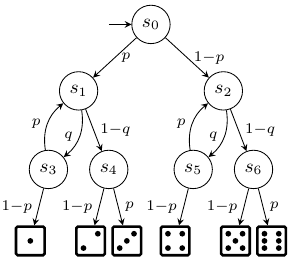
\includegraphics[width=0.5\textwidth]{figures/knuth_die_pq.png}
        \label{fig:knuth-die-pq}
    \end{figure}
\end{example}

\subsection{Parameter synthesis of pDTMC}
With a pDTMC represents a class of DTMC, we concerns of instantiated DTMC which satisfy a certain property of interest.
\begin{definition}{Parameter synthesis (Katoen 2016)\cite{katoen2016probabilistic}} Given a
    parametric DTMC $\mathcal{M}_\theta = (S, \theta, \mathbf{P}, \iota_{init}, AP, L)$ and a
    reachability property $\Phi$, find a set of parameter values $\theta$ such that
    $\mathcal{M}_\theta \models \Phi$.
\end{definition}
Katoen \cite{katoen2013model} summarizes the following methods on parameter synthesis of pDTMC:
\begin{enumerate}
    \item \textit{Computing symbolic reachability probabilities}: using states elimination to obtain symbolic
          rational function of a reachability property \cite{daws2004symbolic}
          \cite{hahn2011probabilistic}.
    \item \textit{Candidate region generation and checking}: partition the parameter space into \textit{safe}
          and \textit{unsafe} regions using non-linear interval arithmetic
          \cite{kwiatkowska2006symmetry}.
    \item \textit{Parameter lifting} is another parameter space partitioning method; it introduces
          new transitions into the original pDTMC through \textit{relaxation} and
          \textit{substitution}. The procedure results in a non-parametric transition system with
          transition labels are bounds from given intervals. The region is then checked using
          candidate region generation and checking method.
\end{enumerate}
In this thesis we use only symbolic model checking \cite{daws2004symbolic}.
\begin{example}{Parametric Knuth's die}
    We continue the example with Knuth die model $\mathcal{M}_{p}$. Assume the
    \begin{lstlisting}
        P(F "1") = (p^2*q+(-1)*p*q)/(p*q+(-1))
        P(F "2") = ((p)^2 * (q+(-1)))/(p*q+(-1))
        P(F "3") = (-1 * ((p) * (p+(-1)) * (q+(-1))))/(p*q+(-1))
        P(F "4") = (-1 * (p^2*q+(-1)*p*q))/(p*q+(-1)*p+1)
        P(F "5") = (p^2*q+(-2)*p*q+q)/(p*q+(-1)*p+1)
        P(F "6") = (-1 * ((p+(-1))^2 * (q+(-1))))/(p*q+(-1)*p+1)
    \end{lstlisting}
\end{example}
With the symbolic rational function $f_\Phi(\theta)$ of $\Phi$ obtained, we assign a parameter value
to $\theta$, then replace all symbolic parameters by their concrete value to check if
$\mathcal{M}_\theta \models \Phi$.
\begin{example}
    Given a pDTMC of Knuth die $\mathcal{M}_{(p,q)}, (p,q)\in[0,1]\times[0,1] $ and a reachability
    property $\Phi = P_{\geq 0.2} (\texttt{F "one"})$, synthesize parameter $(p,q)$ so that
    $\mathcal{M}_{(p,q)} \models \Phi$. A simple Monte-Carlo search on parameter space gives the
    following satisfying points:
    \begin{figure}[H]
        \centering
        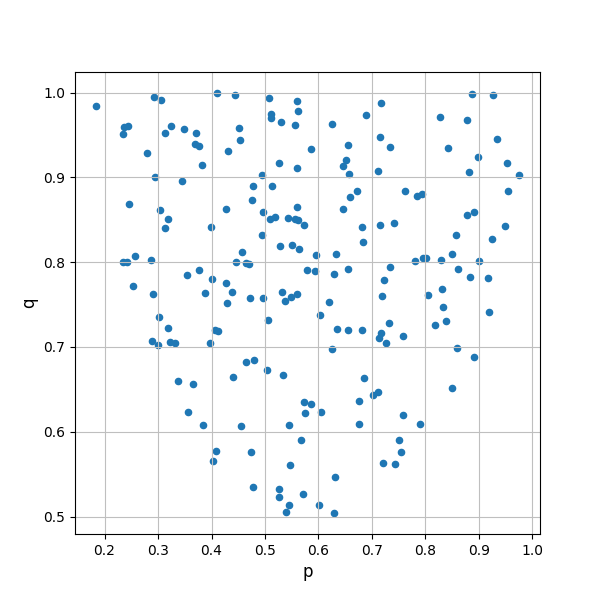
\includegraphics[width=0.5\textwidth]{figures/knuth_die_trueparams.png}
        \label{fig:knuth-die-pq-trueparams}
    \end{figure}
\end{example}

\subsection{Summary}
In this chapter we introduce the essential theoretical concepts on discrete-time models,
probabilistic temporal logic, and parameter synthesis problem. However, the parameter synthesis
methods presented exhaustively search on parameter space for satisfying parameter values. In the
next chapter, we present Bayesian inference methods for later construction of data-informed
parameter synthesis frameworks.